\begin{pro}
  What is the degree of each of the following types of numerical quadrature rules?
  \begin{itemize}
  \item[(a)]
    An $n$-point Newton-Cotes rule,
    where $n$ is odd

  \item[(b)]
    An $n$-point Newton-Cotes rule,
    where $n$ is even

  \item[(c)]
    An $n$-point Gaussian rule

  \item[(d)]
    What accounts for the difference between the answers to parts a and b?

  \item[(e)]
    What accounts for the difference between the answers to parts b and c?
  \end{itemize}
\end{pro}

\begin{sol}
  \begin{itemize}
  \item[(a)]
    $n$.

  \item[(b)]
    $n-1$.

  \item[(c)]
    $2n-1$.

  \item[(d)]
    The difference is due to cancellation of positive and negative errors,
    as illustrated for the midpoint and Simpson's rules in the following figure,
    which, on the left, shows a linear polynomial and
    the constant function interpolating it at the midpoint and,
    on the right, a cubic and the quadratic interpolaing it at the midpoints
    and endpoints.
    Integration of the linear polynomial by the midpoint rule yields
    two congruent triangles of equal area.
    The inclusion of one of the triangles compensates exactly for the
    omission of the other.
    A simiar phenomenon occurs for the cubic polynomial,
    where the two shaded regions also have equal areas,
    so that the addition of one compensates for the subtraction of the other.
    Such cancellation does not occur,
    however,
    for an $n$-point Newton-Cotes rule if $n$ is even.
    \begin{figure}[H]
      \centering
      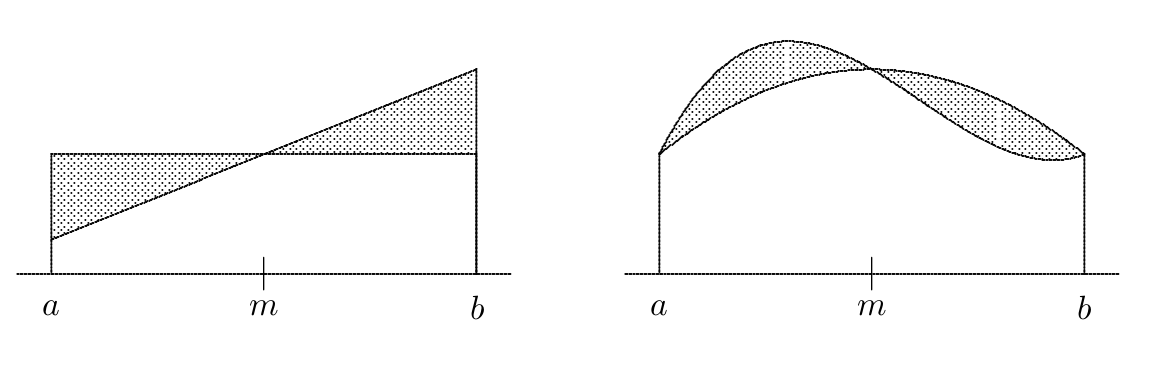
\includegraphics[scale=0.25]{Newton-Cotes.png}
      \caption{Cancellation of errors in midpoint (left) and Simpson (right) rules.}
    \end{figure}

  \item[(e)]
    \begin{itemize}
      \item
    In Newton-Cotes rules,
    the $n$ nodes are prespecified and the $n$ corresponding weights
    are then optimally chosen to maximize the degree of the
    resulting quadrature rules.
    With only $n$ parameters free to be chosen,
    the resulting degree is generally $n-1$.
  \item
    In Gaussian rule,
    the locations of the nodes are also freely chosen,
    then there are $2n$ free parameters,
    so that a degree of $2n-1$ is achievable.
  \end{itemize}
\end{itemize}
\end{sol}
%%% Local Variables:
%%% mode: latex
%%% TeX-master: "../hw4"
%%% End:
